%!TEX root = main.tex

\section{Data and Experiments}
\label{sec:experiments}
In this section we  evaluate our strategies for drivers 
in practice. First, we discuss how we collect and combine the appropriate data 
from multiple data sources. Then, we perform a comprehensive experimental study
that reveals the benefits of being strategic for the drivers and provides
specific insights as to how drivers can maximize their earnings.

\subsection{Data collection and preparation}
In order to evaluate our strategies, we need to construct 
time-evolving matrices 
{\empiricaltransitionmatrix}, {\traveltimematrix} and {\rewardsmatrix} as defined in Section~\ref{sec:problem_setup},
and {\countmatrix} as defined in Section~\ref{sec:sensitivity}.
For this we use two data sources: (1) the NYC taxi rides 
dataset~\footnote{\url{http://www.nyc.gov/html/tlc/html/about/trip_record_data.shtml}} and
(2) information we obtain from the Uber platform via queries to the Uber API.

\begin{figure}
	\centering
	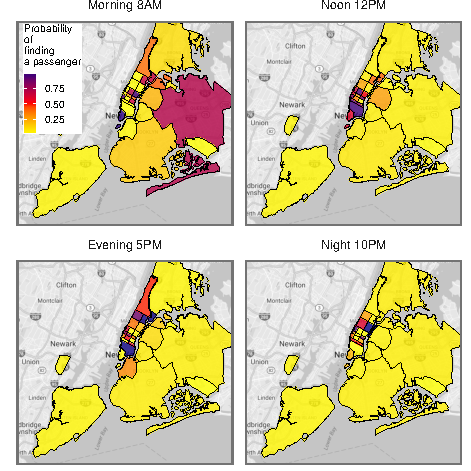
\includegraphics{figures/successful_heatmap.pdf}
	\caption{Probability of finding a passenger in 10 minutes across NYC zones at different times of the day.}
	\label{fig:successful_heatmap}
\end{figure}


\spara{Forming time-evolving matrices {\countmatrix} and {\empiricaltransitionmatrix}:}
Our starting point is the the NYC taxi rides dataset, which
%%\footnote{\url{http://www.nyc.gov/html/tlc/html/about/trip_record_data.shtml}}. 
contains yellow street-hail taxi records with fields capturing pick-up and drop-off dates/times, 
location co-ordinates, trip distances and fares. 
{\bf{What time period?  How many rides?}}
Each taxi record is accompanied with taxi location ID for the pick-up and drop-off locations. 
Each location ID is associated with one of 29 non-overlapping city zones -- defined in the
dataset.  While the set of taxi rides is undoubtedly produced from a different ridership than Uber
rides, resulting in differences of geographical diversity, demographics, and timing, than Uber rides, 
it nonetheless provides a useful baseline that reflects many of the broader dynamics of ridership in 
NYC over space and time.  Thus we this to build count and frequency input matrices, as follows.


We divide each 24-hour day of the week into 144 time-slices of duration 10 minutes each, indexed by their start 
time.  To model traffic demand in the city at time $t$, the $c(i,j)$ entry of the count matrix $\countmatrix^t$ is the total 
number of rides from zone $i$ to zone $j$ in a 30-minute long time window centered at time $t$, {\bf is this right?
summed over all rides in that time period in the dataset}.  In other words, $c(i, j)$ for the time slot corresponding
to [10:40, 10:50] on a Wednesday is a count of all rides from $i$ to $j$ that were initiated between 10:30 and 11:00 
on any Wednesday in the dataset.

The empirical transition matrix $\empiricaltransitionmatrix^t$ is now formed as follows.
 Every diagonal entry of the count matrix $\countmatrix^t$ is zero, as there are no passenger rides within same zone. 
{\bf Why?  Are they not in the dataset, or is this disallowed in our model?}.
However, the empirical transition matrix $\empiricaltransitionmatrix^t$ described in Section \ref{sec:problem_setup} assumes that the diagonal entries $f(i,i)$ denote the probabilities of a driver not finding a passenger in zone $i$ in the time-slice $t$. We compute these probabilities below.

%\spara{Modeling successful passenger pickup}:
Let $N(\passengerarrivalrate)$ and $N(\driverarrivalrate)$ denote the number of passenger and driver arrivals in zone $i$ in one time unit, with Poisson arrival rates {\passengerarrivalrate} and {\driverarrivalrate} respectively. Assuming that passenger and driver arrivals are independent Poisson processes, the random variable $K = N(\passengerarrivalrate) - N(\driverarrivalrate)$ follows a Skellam distribution 
%and can be depicted by states of a Markov Chain 
such that:
\begin{equation}
\Pr[K=k] = e^{-(\passengerarrivalrate + \driverarrivalrate)} \bigg(\frac{\passengerarrivalrate}{\driverarrivalrate}\bigg) I_k\big(2 \sqrt{\passengerarrivalrate \driverarrivalrate}\big)
\end{equation}
where $I_k(z)$ is the modified Bessel function of the first kind\footnote{Although, for simplicity, we assume the independence of the passenger and driver arrival processes, we can also accommodate correlated processes with slight modification.}.

Whenever %the Markov Chain is in a non-positive state, 
$K<0$, there are more drivers than passengers in a given zone. We assume the worst case scenario in which a driver joins the corresponding FIFO queue at the last spot. Hence, for a state $k \leq 0$, the driver has to wait for $(|k| + 1)$ passenger arrivals in a unit time for a successful passenger pickup. The probability of a successful passenger pickup can be expressed as,
\begin{equation}
\Pr[N(\passengerarrivalrate) = |k| + 1] = \frac{\passengerarrivalrate^{\big(|k|+1\big)} e^{-\passengerarrivalrate}}{\big(|k| + 1\big)!}
\end{equation}
Thus, we can express a diagonal entry $f^t(i,i)$ of empirical transition matrix as follows,
\begin{equation}
f^t(i,i) = 1 - \sum_{k \leq 0} \Pr[K = k] \times \Pr[N(\passengerarrivalrate) \geq |k| + 1]
\end{equation}
To maintain the right stochasticity of {\empiricaltransitionmatrix}, every other entry 
$f^t(i,j)$ is calculated as,
\begin{equation}
f^t(i,j) = (1 - f^t(i,i)) \times \frac{c^t(i,j)}{\sum_{j}c^t(i,j)}. 
\end{equation}
The matrix $\empiricaltransitionmatrix^t$, built in this manner satisfies all our assumptions and can be used as input to our algorithms. 

Figure \ref{fig:successful_heatmap} shows an example of varying probabilities of successful pickups in different zones at various times of the day. As expected, we see that the probability of a successful pickup is higher outside Manhattan in the morning, and this trend reverses in the evening.

\spara{Forming time-evolving matrices {\traveltimematrix}, {\rewardsmatrix}:} Since information about travel times 
and rewards was not available on the NYC Taxi dataset we invoked the Uber API in order
to obtain this information.
The HTTP-based Uber API allows third-party developers to retrieve information about Uber. For our study, the most relevant feature of the API is \texttt{estimates/price}. It takes longitude and latitude of pick-up and drop-off locations and returns price estimates for all types of Uber products - UberX, UberXL and UberBlack. Along with the price estimates, it also provides the active surge multiplier rate at the pick-up location at the time of query. For the purpose of this study, we only focus on UberX, the most popular Uber product. We also use the \texttt{/products} endpoint to get information regarding the base fare, minimum fare, cost per minute and cost per unit distance for UberX. However, none of the Uber API endpoints provide information about the supply of UberX drivers or demand of passengers; we use this information from the
NYC taxi rides dataset.

To create a representative sample of data, our strategy relies on ``recreating" NYC taxi rides virtually on the Uber platform. 
We use the price estimates endpoint to query rides from exact same pick-up to drop-off locations at the exact same time of the 
day on the same calendar date, but one year later i.e, a real recorded ride from November 10, 2015 was virtually recreated on November 10, 2016. However, Uber imposes a rate limit of 1,000 API requests per hour per account. To respect these API limits, we randomly sample rides between each pair of zones in the city every 15 minutes. We assume that price estimates, travel times and distance of preferred travel paths by drivers do not vary significantly in 15 minutes. Chen {\etal}~\cite{chen2015peeking} have observed that 90\% of the surges on Uber platform have durations as multiples of 5 minutes. Hence, every 5 minutes, we also query the surge multiplier active within each zone.

%Although the \texttt{estimates/time} endpoint of the Uber API returns the estimated waiting time for a passenger at a particular location, it provides no information on the supply of UberX cars in its neighborhood. Consequently, we do not possess an exact estimate of the time spent by an Uber driver waiting for a passenger in a particular zone. 
%In the next section we discuss how we get an estimate of that quantity.
%
%However, in the next section, we provide a methodology to compute a conservative estimate of the driver waiting time in a particular zone at any time of the day using the successful passenger pick-up information from the NYC taxi rides dataset.

Using this aforementioned approach, we collected data for a period of 6 months, recreating rides from October, 2015 until March, 2016. However, due to seasonality of the data, we provide experimental results for one week starting October 18, 2015\footnote{Our results do not vary qualitatively across different weeks.}.


Using the same time-slicing as we described in the previous paragraph and the same
29 city zones, the
travel time matrix $\traveltimematrix^t$ and rewards matrix $\rewardsmatrix^t$ entries contain the average travel times and average rewards of traveling between two zones
as computed by the above data-collection process. Note that each entry of the {\rewardsmatrix} matrix represents net reward, calculated after taking into account the surge information, along with driver expenses and Uber's share. %of earnings.


\iffalse
\subsection{Data collection}
\label{sec:data}
To evaluate our methods, we need a representative sample of taxi rides data. To obtain this data, we strategically sample rides from the publicly available NYC taxi rides 
dataset~\footnote{\url{http://www.nyc.gov/html/tlc/html/about/trip_record_data.shtml}} and recreate them on the Uber platform using Uber API queries.

\spara{The Uber API}: 
The HTTP-based Uber API allows third-party developers to retrieve information about Uber. For our study, the most relevant endpoint of the API is \texttt{estimates/price}. It takes longitude and latitude of pick-up and drop-off locations and returns price estimates for all types of Uber products - UberX, UberXL and UberBlack. Along with the price estimates, it also provides the active surge multiplier rate at the pick-up location at the time of query. For the purpose of this study, we only focus on UberX, the most popular Uber product. We also use the \texttt{/products} endpoint to get information regarding the base fare, minimum fare, cost per minute and cost per unit distance for UberX. However, none of the Uber API endpoints provide information about the supply of UberX drivers or demand of passengers. To overcome this obstacle, we leverage the NYC taxi rides dataset.

\spara{NYC taxi-rides dataset}:
NYC taxi rides dataset\footnote{\url{http://www.nyc.gov/html/tlc/html/about/trip_record_data.shtml}} for the year 2015 contains yellow street-hail taxi records with fields capturing pick-up and drop-off dates/times, location co-ordinates, trip distances and fares. Each taxi record is accompanied with taxi location ID for the pick-up and drop-off locations. We use these location IDs to divide the city into a set of 29 non-overlapping zones.

\spara{Querying the Uber API}:
To create a representative sample of data, our strategy relies on `recreating' NYC taxi rides virtually on the Uber platform. We use the price estimates endpoint to query rides from exact same pick-up to drop-off locations at exact same time of the day on same calendar date, but exactly one year later i.e, a real recorded ride from 2015 is virtually recreated in 2016. However, Uber imposes a rate limit of 1,000 API requests per hour per account. To respect these API limits, we randomly sample rides between each pair of zones in the city every 15 minutes. We assume that price estimates, travel times and distance of preferred travel paths by drivers do not vary significantly in 15 minutes. Chen {\etal}~\cite{chen2015peeking} have observed that 90\% of the surges on Uber platform have durations as multiples of 5 minutes. Hence, every 5 minutes, we also query the surge multiplier active within each zone.

Although the \texttt{estimates/time} endpoint of the Uber API returns the estimated waiting time for a passenger at a particular location, it provides no information on the supply of UberX cars in its neighborhood. Consequently, we do not possess an exact estimate of the time spent by an Uber driver waiting for a passenger in a particular zone. 
In the next section we discuss how we get an estimate of that quantity.
%
%However, in the next section, we provide a methodology to compute a conservative estimate of the driver waiting time in a particular zone at any time of the day using the successful passenger pick-up information from the NYC taxi rides dataset.

Using aforementioned approach, we collected data for a period of 6 months, recreating rides from October, 2015 till March, 2016. However, due to the periodicity of the data, we provide experimental results for one week starting October 18, 2015\footnote{Our results do not vary qualitatively across different weeks.}.

\subsection{Experimental setup}
In this section, we describe how the collected data can be used for modeling the dynamics of the city as well as an individual driver, as described in Section \ref{sec:problem_setup}.


\spara{Modeling the city}:
We divide each 24-hour day of the week in 144 time-slices of duration 10 minutes each, indexed by their start time. While modeling the city, the $c(i,j)$ entry of the count matrix $\countmatrix^t$ is the total number of rides from zone $i$ to zone $j$ in a 30-minute long time window centered around time $t$. 

\begin{figure}
	\centering
	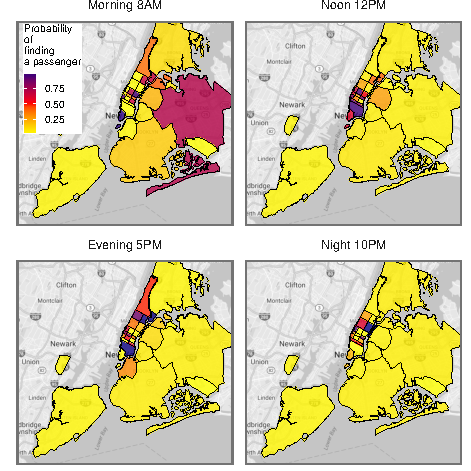
\includegraphics{figures/successful_heatmap.pdf}
	\caption{Estimated probability of finding a passenger within 10 minutes across NYC zones at different times of day.}
	\label{fig:successful_heatmap}
\end{figure}

Similarly, travel time matrix $\traveltimematrix^t$ and rewards matrix $\rewardsmatrix^t$ entries contain the average travel times and average rewards of traveling between two zones. Recall that each entry of the {\rewardsmatrix} matrix represents the net reward, calculated after taking into account the surge multiplier, estimated driver expenses and Uber's share of the earnings.



Now, we describe the formation of the empirical transition matrix $\empiricaltransitionmatrix^t$. Every diagonal entry of the count matrix $\countmatrix^t$ is zero, as there are no passenger rides within same zone. However, the empirical transition matrix $\empiricaltransitionmatrix^t$ described in Section \ref{sec:problem_setup} assumes that the diagonal entries $f(i,i)$ denote the probabilities of a driver not finding a passenger in zone $i$ in the time-slice $t$. Hence, to form the empirical transition matrix, we first normalize the observed count matrix such that each of its rows sum up to 1 and call this matrix $\countmatrix^\prime$. 
In the following section, we describe the formation of empirical transition matrix $\empiricaltransitionmatrix^t$, using the matrix $\countmatrix^\prime$.

%\spara{Modeling successful passenger pickup}:
Let $N(\passengerarrivalrate)$ and $N(\driverarrivalrate)$ denote the number of passenger and driver arrivals in zone $i$ in one time unit, with Poisson arrival rates {\passengerarrivalrate} and {\driverarrivalrate} respectively. Assuming that passenger and driver arrivals are independent Poisson processes, the random variable $K = N(\passengerarrivalrate) - N(\driverarrivalrate)$ follows a Skellam distribution 
%and can be depicted by states of a Markov Chain 
such that:
\begin{equation}
\Pr[K=k] = e^{-(\passengerarrivalrate + \driverarrivalrate)} \bigg(\frac{\passengerarrivalrate}{\driverarrivalrate}\bigg) I_k\big(2 \sqrt{\passengerarrivalrate \driverarrivalrate}\big)
\end{equation}
where $I_k(z)$ is the modified Bessel function of the first kind\footnote{Although, for simplicity, we assume the independence of the passenger and driver arrival processes, we can also accommodate correlated processes with slight modification.}.

Whenever %the Markov Chain is in a non-positive state, 
$K<0$, there are more drivers than passengers in a given zone. We assume the worst case scenario in which a driver joins the corresponding FIFO queue at the last spot. Hence, for a state $k \leq 0$, the driver has to wait for $(|k| + 1)$ passenger arrivals in a unit time for a successful passenger pickup. The probability of a successful passenger pickup can be expressed as,
\begin{equation}
\Pr[N(\passengerarrivalrate) = |k| + 1] = \frac{\passengerarrivalrate^{\big(|k|+1\big)} e^{-\passengerarrivalrate}}{\big(|k| + 1\big)!}
\end{equation}
Thus, we can express a diagonal entry $f(i,i)$ of empirical transition matrix as follows,
\begin{equation}
f(i,i) = 1 - \sum_{k \leq 0} \Pr[K = k] \times \Pr[N(\passengerarrivalrate) \geq |k| + 1]
\end{equation}
To maintain the right stochasticity of {\empiricaltransitionmatrix}, every other entry $f(i,j)$ is calculated as,
\begin{equation}
f(i,j) = (1 - f(i,i)) \times c^\prime(i,j)
\end{equation}
The matrix $\empiricaltransitionmatrix^t$, built in this manner satisfies all our assumptions and can be used in the evaluation of strategies described in previous sections. 

Figure \ref{fig:successful_heatmap} shows an example of varying probabilities of successful pickups in different zones at various times of the day. As expected, we see that the probability of a successful pickup is higher outside Manhattan in the morning, and this trend reverses in the evening.

\fi

\subsection{Experimental results}
\begin{figure*}
	\centering
	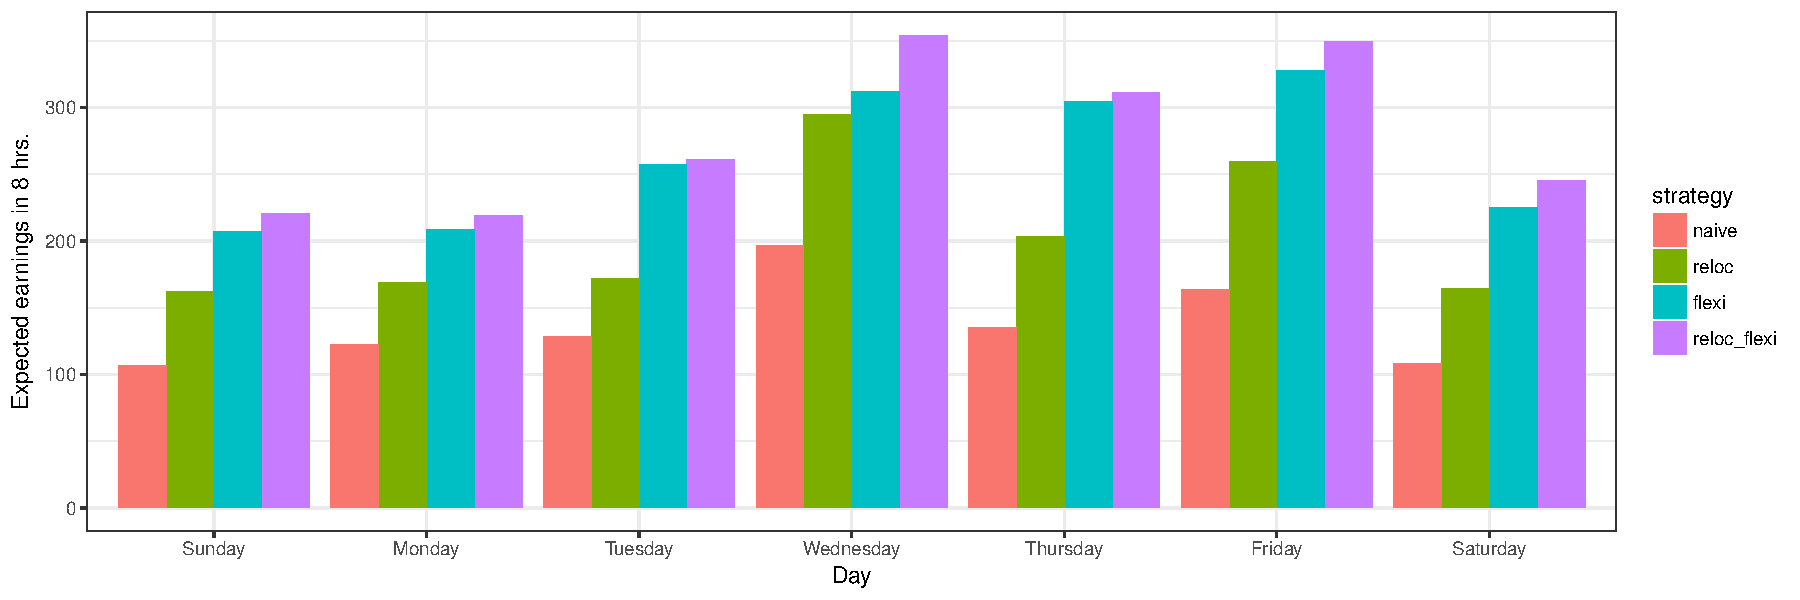
\includegraphics{figures/daily_earnings.pdf}
	\caption{Daily earnings with different strategies}
	\label{fig:daily_earnings}
\end{figure*}

Now, we use the experimental framework from the previous section to evaluate various driver strategies formulated in Section \ref{sec:driver_strategies}.

\spara{Comparison of strategies}: First, we answer the question: \textit{what is the best driver strategy?} Intuitively, it is clear that {\relocationflexible} strategy is the best strategy as it takes advantage of spatial as well as temporal variations in the passenger demand across NYC. In order to verify this intuition, we compare driver earnings across different strategies. Drivers following the {\naive} and the {\relocation} strategies are assumed to drive from 9AM to 5PM, a standard 8 hour workday, while those following the {\flexible} or the {\relocationflexible} strategies drive for a total of 8 hours each day with a flexible schedule.

Figure \ref{fig:daily_earnings} plots the solution to the {\originalproblem} for each of the strategies on different days of the week. We observe that all of the `smart' strategies consistently outperform the {\naive} strategies. The {\relocation} as well as the {\flexible} strategy earnings are more than that of {\naive}. This shows that, indeed, our strategies are able to exploit the spatial and the temporal variation in demand across NYC. As a result, the most general {\relocationflexible} strategy is always the best strategy, with earnings over twice than those from the {\naive} strategy. We also find that, for a part-time Uber driver, it is beneficial to drive midweek from Wednesday to Friday, than during weekends.

Having established that the {\relocation}, {\flexible} and {\relocationflexible} strategies result in higher driver earnings than the {\naive} strategy, in the subsequent sections, we further analyze various aspects related to them.

\spara{Spatial dynamics of strategies}: 
\begin{figure}
	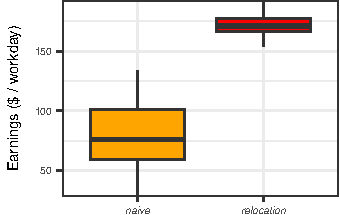
\includegraphics{figures/earnings_heatmap.pdf}
	\caption{Disparity of earnings between {\naive} and {\relocation} strategies}
	\label{fig:earnings_heatmap}
\end{figure}
Here, we attempt to answer the question - \textit{what are the benefits of the {\relocate} action?} Figure \ref{fig:successful_heatmap} already shows the spatial variation in the demand across different NYC zones at different times of the day. Intuitively, this spatial variation can cause a disparity in the driver earnings based upon the zone of the driver. For example, the drivers based in Manhattan should be expected to earn more than those based in Brooklyn due to higher demand in Manhattan. Similarly, at different times of the day, drivers located within different parts of Manhattan itself will earn differently on account of temporal trends.

\begin{figure*}
	\centering
	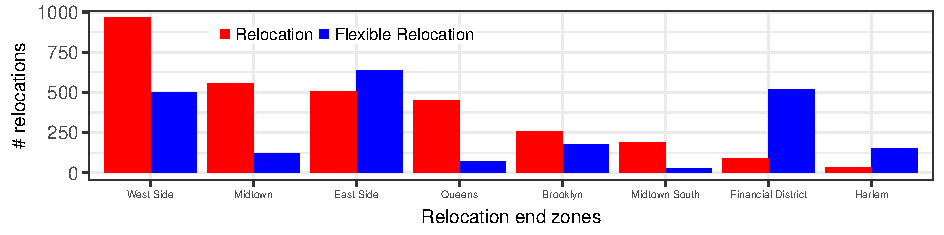
\includegraphics{figures/relocation_endzones.pdf}
	\caption{Contrast between preferred relocation endzones for drivers with 
	{\relocation} and {\relocationflexible} strategies}
	\label{fig:relocation_endzones}
\end{figure*}

The {\relocation} strategy attempts to mitigate the location based inequality in earnings by suggesting optimal relocation actions to drivers at various times of the day. Figure \ref{fig:earnings_heatmap} is a box-plot of earnings from an 8-hour workday for drivers following {\naive} and {\relocation} strategies with different home zones. Not only do we observe that {\relocation} strategy has a higher median than that of the {\naive} strategy, but also, the inter-quartile range (IQR) is significantly narrow\footnote{The lower and upper edges of the boxes in Figure \ref{fig:earnings_heatmap} indicate quartiles Q1 and Q3 respectively, and length of whisker is 1.5 times IQR.}. Thus, we conclude that smart relocations throughout the day prevent a driver from being localized to low-earnings neighborhoods of the city, thereby vastly increasing the earnings. The net increase in earnings due to the {\relocate} action easily compensates for the lost time and the costs associated with the action.

\spara{Temporal dynamics of strategies}: Intuitively, it should be obvious that, on account of periodicity in demand, driver earnings strongly depend on the time of the day when they are driving. We have also established via Figure \ref{fig:daily_earnings} that both of the flexible schedule strategies outperform their fixed schedule counterparts. Now, we explore the question \textit{what is the best time of the day to drive in order to maximize earnings?} To answer this question, we simulate 1000 drivers each for the {\flexible} and {\relocationflexible} strategies. Each of the drivers is randomly assigned a home zone. Furthermore, we solve the {\originalproblem} problem for both the strategies and create a recommended plan of action for the simulated drivers. Thus, at every step of simulation, a driver undertakes the action recommended by the strategy, depending upon the location, time of the day and the budget left.

\begin{figure}[H]
	\centering
	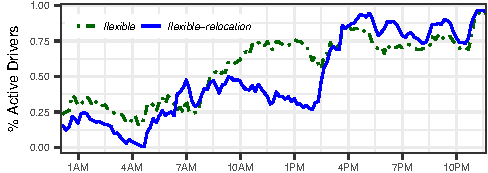
\includegraphics{figures/simulated_schedules.pdf}
	\caption{Active drivers with {\flexible} and {\relocationflexible}
	strategies at different times of the day.}
	\label{fig:simulated_schedules}
\end{figure}

In Figure \ref{fig:simulated_schedules} we plot the percentage of simulated drivers driving in the city at different times of the day. We observe a noticeable difference between the `preferred' driving schedules as output by the strategies and consequently followed by the simulated drivers. In particular, a high percentage of {\flexible} schedule drivers are active during the standard working hours of the day from 9AM to 6PM. In contrast, the {\relocationflexible} driver schedules exhibit two distinct peaks corresponding to the morning and the evening peak hour demand. Furthermore, over 50\% of {\relocationflexible} drivers use their driving budget in the later half of the day starting approximately at 3PM, continuing through till midnight. 

We also know that the observed differences in the schedules of two strategies are on account of the {\relocate} action. Hence, we can also conclude that the {\relocate} action is more effective in the evening hours, thereby prompting higher active percentages of {\relocationflexible} drivers then.

\spara{Preferred relocation zones}: Simulated drivers also allow us to compare the {\relocate} actions between drivers following {\relocation} strategy and those following {\relocationflexible} strategy. The popular destinations of {\relocate} actions for drivers following the two strategies are plotted in Figure \ref{fig:relocation_endzones}. We observe a contrast between the preferred relocation zones for drivers of either strategies. Drivers following the {\relocation} strategy predominantly relocate themselves to the center of Manhattan. In contrast, the drivers following {\relocationflexible} strategy do not exhibit a clear most preferred relocation destination. Furthermore, the number of relocations by the {\relocation} strategy drivers vastly outnumber those by the {\relocationflexible} strategy drivers. This presumably results from the freedom of flexible work schedule, allowing them to drive during the hours of higher demand, reducing the number of {\relocate} actions. 

\subsection{Surge Chasing}
\begin{figure}
	\centering
	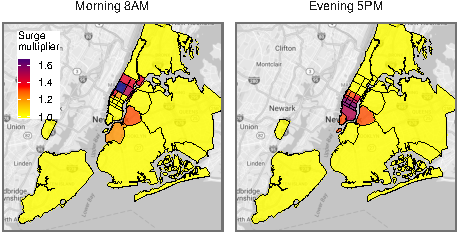
\includegraphics{figures/surge_heatmap.pdf}
	\caption{Active surge multiplier across NYC zones at different times of the day.}
	\label{fig:surge_heatmap}
\end{figure}
Now that we have an understanding about the dominant aspects of various driver strategies, we turn our attention to surge pricing. Surge pricing was a controversial feature of the Uber platform\footnote{Uber has stopped displaying the `surge multiplier' prominently in its customer app since June 2016, instead now it displays price estimates after accounting for the surge~\cite{surge}.} aimed at matching supply with passenger demand by increasing prices at times of high-demand. According to Uber, it encourages drivers to start driving during the peak hours in order to efficiently meet demand with supply, albeit at a higher cost to passenger, in turn leading to higher driver earnings. It also decreases demand as the price sensitive customers drop out. In fact, Uber prominently displays to drivers on their Partner App, the information regarding surge multiplier in different geographical neighborhoods in form of a heatmap. Figure \ref{fig:surge_heatmap} shows the active surge multiplier across different neighborhoods of NYC at different times of the day. This information is readily available to the drivers, however, due to uncertainty in the duration of surges as well as the proprietary nature of Uber's surge pricing algorithm, it is unclear whether drivers should relocate themselves to surging areas consistently in order to maximize their earnings. Using our information about surge multipliers, we are in a position to answer the question-- \textit{Should drivers engage in surge chasing?}
\begin{figure}[H]
	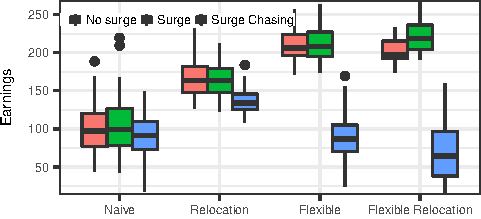
\includegraphics{figures/simulated_earnings.pdf}
	\caption{Simulated earnings for drivers across different strategies.}
	\label{fig:simulated_earnings}
\end{figure}
In order to do so, we evaluate earnings of simulated drivers in three scenarios viz., `no surge' - when we disable the surge multiplier, `surge' - when surge multiplier is used while calculating earnings, and `surge chasing' wherein a driver `chases surge' i.e, a driver located in a non-surging zone always relocates to the zone with highest surge multiplier. Simulated driver earnings in these three scenarios for each of the strategies are shown in Figure {\ref{fig:simulated_earnings}}. We observe that `surge chasing' leads to lower earnings irrespective of the strategy being followed. Figure \ref{fig:simulated_earnings} reinforces our previous observation regarding high variance of the {\naive} strategy. At times, drivers following the {\naive} strategy with surge multiplier enabled may earn less than when it is disabled. For other strategies, `surge chasing' consistently fails to provide any tangible benefits as compared to following the pre-determined strategy. We conclude that actively chasing the surge is an ill-advised strategy and may lead to losses. Furthermore, surges last for short durations and an unsuccessful surge chase may land a driver in sub-optimal location with respect to longer term earnings maximization. 

\subsection{Effect of uncertainty} 

All the experiments described in previous section indicate that our strategies always outperform a {\naive} strategy, the most prevalent strategy among Uber drivers. However, it is worth noting that our strategies are evaluated based on historical data. Consequently, such strategies can be highly sensitive to underlying parametric uncertainty, in form of perturbed empirically observed transition matrices. We can recommend our strategies to drivers only if they outperform the {\naive} strategy in even in the presence of such perturbations. Hence, using the framework developed in Section \ref{sec:sensitivity}, we solve the {\robustproblem} problem for each of the four strategies for increasing levels of uncertainty ($\alpha$).

Figure \ref{fig:uncertainty_evolution} shows the results of increasing uncertainty on the earnings of drivers following each of the four strategies. We find that the {\relocation}, {\flexible} and {\relocationflexible} strategies are more tolerant to uncertainty in transition matrices. Crucially, even with 99\% uncertainty, the {\relocationflexible} strategy outperforms the {\naive} strategy with no uncertainty in form of \$100 extra earnings in a typical workday. This observation supports our claim that strategies based on historical data can improve driver earnings on the on-demand ridesharing platforms. 

\begin{figure}[H]
	\centering
	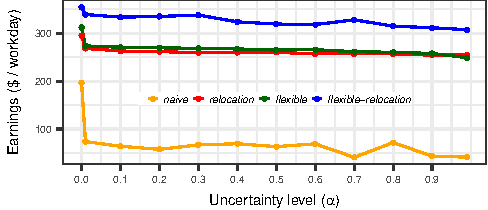
\includegraphics{figures/uncertainty_evolution.pdf}
	\caption{Sensitivity to uncertainty in parameters.}
	\label{fig:uncertainty_evolution}
\end{figure}

% \subsection{\textsc{RewardsMatrix}}

% The data gathered in the previous section gives us a matrix of driver earnings, \matr{E}, from passengers while traveling between any two zones in the city. We also get a costs matrix, \matr{C}, whose each entry, $c(i,j) \leq 0$, denotes the sundry expenses of traveling from zone $i$ to zone $j$, dependent on distance and traffic at the given time. The travel costs can result in negative net rewards in the {\gohome} and {\relocate} actions, violating the assumption from Section \ref{sec:problem_setup} that $r(i,j) \geq 0$. In this section, we describe the construction of \textsc{RewardsMatrix}, {\rewardsmatrix}, corresponding to each driver action compliant with our assumptions.

% \subsubsection{\textsc{Modifying the CostsMatrix}}
% If $min\_cost$ is the minimum entry in the matrix \matr{C}, each entry of the modified costs matrix, \matr{C'} is calculated as,
% \begin{equation}
% c'(i,j) = c(i,j) - min\_cost
% \end{equation}
% As a result of the above modification, $\forall i,j : c'(i,j) \geq 0$.

% \subsubsection{\textsc{RewardsMatrix}}
% In order to be compliant with the assumption in Section \ref{sec:problem_setup}, we define two kinds of \textsc{RewardsMatrix}, one for the action {\getpassenger} and another for the actions {\gohome} and {\relocate}.

% \begin{itemize}
% 	\item For the {\getpassenger} action, we define the rewards matrix as,
% 	\begin{equation}
% 		r(i,j) = e(i,j) + c'(i,j) 
% 	\end{equation}
% 	\item For the {\gohome} and {\relocate} actions, the rewards matrix is same as the modified costs matrix.
% 	\begin{equation}
% 		r(i,j) = c'(i,j)
% 	\end{equation}
% \end{itemize}
% In both cases, we set the diagonal entries of the matrix to zero i.e., $\forall i: r(i,i) = 0$.

% It should be noted that this modification does not affect the optimal action choice in any strategy. It merely ensures that the input vectors to the Bisection Algorithm from Section \ref{sec:sensitivity} are always non-negative vectors. Furthermore, while calculating the actual {\totalexpectedearnings} of a driver, we can backtrack these modifications.

% \subsection{\textsc{Comparing robust and nominal strategies}}
% In this section, we compare various strategies. When we choose, $\beta = \betamax$, there is no uncertainty, and we get solution computed via the classical Bellman recursion; referred to as nominal strategy. The robust strategy corresponds to solving the MDP with varying values of $\beta$.

% \subsection{\textsc{Effect of Inaccuracy is uncertainty level}}
% The previous section assumes that, in the robust case, we are able to estimate exactly the precise value of the uncertainty level. In practice, the parameter $\beta$ also has to be estimated. In this section, we study the sensitivity of the robust approach with respect to inaccuracies in the uncertainty parameter $\beta$.
